\chapter{Introduction}
\label{ch:introduction}

Each chapter of this report lives in its own file in the \texttt{chapters/}
folder and is pulled in with \verb|\include|. Errors are reported against
the right file, and double-clicking the PDF opens the correct chapter.

Typesetting systems have a long history~\cite{knuth1984,lamport1994}.
\Cref{ch:methods} describes the method, \cref{ch:results} presents results
and \cref{ch:conclusion} concludes.

\section{Motivation}
A landscape picture is shown in \cref{fig:intro}.

\begin{figure}[htbp]
  \centering
  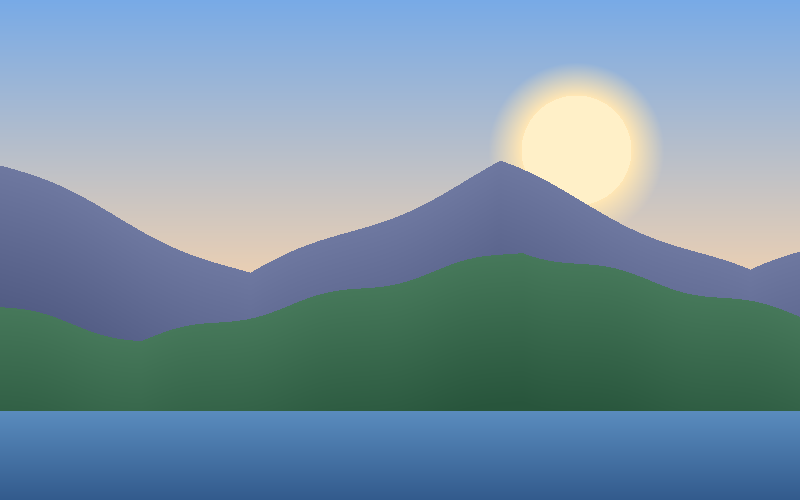
\includegraphics[width=0.6\linewidth]{landscape.png}
  \caption{An example figure in the introduction.}
  \label{fig:intro}
\end{figure}
